
\chapter{Revisión Bibliográfica}

\section{Mecanismos de defensa en plantas.}

Las plantas juegan un papel fundamental en la sostenibilidad de la vida en la Tierra, al convertir en nutrientes la energía solar, por lo que son la fuente vital de la mayoría de los organismos. Continuamente se enfrentan a condiciones adversas tanto bióticas (bacterias, virus, viroides, hongos, protistas, micoplasmas e invertebrados), como abióticas (sequías, temperaturas extremas, presencia de metales pesados, entre otros), frente a las cuales se desencadenan respuestas de defensa. Para hacer frente a estas amenazas, las plantas poseen un sistema de defensa altamente sofisticado, el cual, como el sistema inmune en animales, reconoce las moléculas no propias o señales emitidas por las células dañadas, y responden por activación de una efectiva respuesta inmune contra los organismos invasores \citep{jones2006plant, howe2008plant}.

\subsection {Defensa ante ataque de pat\'ogenos.}

Los mecanismos de defensa de las plantas frente al ataque de pat\'ogenos pueden ser clasificados en dos categor\'ias: defensas constitutivas o preexistentes y defensas inducidas \citep{mithofer2012plant}.

\subsubsection{Defensas constitutivas o preexistentes.}

Los mecanismos de defensa constitutivos, siempre est\'an presentes en las plantas. Estos mecanismos incluyen características estructurales y productos del metabolismo secundario que poseen propiedades antimicrobianas. Estos metabolitos secundarios pueden existir en formas biológicamente activas o pueden ser almacenados en compartimentos celulares espec\'ificos como precursores inactivos que se activan enzimáticamente en respuesta a ataques de patógenos o daños tisulares \citep{mithofer2016general}.
		
\subsubsection{Defensas inducidas.}

A diferencia de las defensas constitutivas, la activaci\'on de los mecanismos de defensa inducida dependen del reconocimiento del pat\'ogeno por la planta.\\ 

La Inmunidad Desencadenada por Patrones (PTI, por sus siglas en ingl\'es) constituye la primera línea de defensa de las plantas frente al ataque por patógeno, y tiene lugar a través del reconocimiento de Patrones Moleculares Asociados a Patógenos (PAMP/MAMPs, por sus siglas en ingl\'es) relativamente conservados, que interact\'uan con  Receptores de Reconocimiento de Patrones (PRRs, por sus siglas en ingl\'es) ubicados en la superficie celular \citep{trda2015perception}. Sin embargo, en numerosas ocasiones, existen patógenos que son capaces de emitir moléculas efectoras que rompen esta primera línea de defensa \citep{de2010conserved, bardoel2011molecular}. Frente a estos patógenos exitosos, las plantas tienen una segunda línea de defensa, donde proteínas de Resistencia (R) median el reconocimiento de estos efectores específicos del atacante, lo que conlleva a una Inmunidad Desencadenada por Efectores (ETI, por sus siglas en inglés) \citep{pieterse2009networking}.\\

La PTI conduce a la fortificación de la pared celular, induce la expresión de genes que codifican proteínas antimicrobianas o enzimas que participan en vías de síntesis de compuestos antimicrobianos y estimula la producción de Especies Reactivas del Oxígeno (ROS, por sus siglas en inglés). La ETI también conduce a muchas de estas respuestas, pero es usualmente más fuerte que la PTI ya que tiene un efecto nocivo directo sobre el patógeno e induce genes de defensa \citep{grant2000role}. A menudo culmina en un proceso donde se produce la muerte celular programada que se conoce como Respuesta Hipersensible (HR, por sus siglas en inglés) \citep{taiz2017fisiologia}. \\

\subsection{Defensas ante estr\'es abi\'otico.}

Las plantas se encuentran frecuentemente expuestas a condiciones ambientales desfavorables que afectan su crecimiento, desarrollo y reproducci\'on. Entre estas condiciones se encuentran: inundaciones, sequ\'ias, temperaturas extremas, salinidad excesiva de los suelos, disposici\'on inadecuada de nutrientes y el exceso o deficiencia de luz. Como resultados directos de la influencia del estr\'es, o de los da\~nos que produce, se desencadena un amplio rango de respuestas vegetales que puede modificar la expresi\'on gen\'etica y el metabolismo celular \citep{buchanan2015biochemistry}. \\

Los mecanismos de resistencia al estr\'es abi\'otico pueden ser agrupados en dos categor\'ias: mecanismos de evasi\'on, que previenen la exposici\'on al estr\'es, y los mecanismos de tolerancia, que le permiten a la planta resistir a este tipo de estr\'es. Algunos mecanismos de tolerancia como el cierre de los estomas, las espinas reflectoras de la luz y las ra\'ices profundas, son rasgos constitutivos que est\'an presentes en plantas, independientemente de la presencia o no de condiciones ambientales desfavorables. Existen, adem\'as, otros mecanismos de resistencia que son adquiridos a través del proceso de aclimatación, donde las plantas alteran su homeostasis, en respuesta a los cambios de los factores ambientales \citep{buchanan2015biochemistry}. \\

\subsection{Defensa hormonal.}

Las hormonas vegetales son moléculas de señalización que están presentes en muy pequeñas cantidades. La sensibilidad del tejido a estas y los cambios en la concentración hormonal median procesos de desarrollo y las respuestas de defensa frente a factores ambientales \citep{verma2016plant}.

\subsubsection{Brasinoesteroides (BRs).}

En los inicios de 1960, se pensaba que el rápido crecimiento y germinación de granos de polen estaban asociados a la presencia de un promotor del crecimiento \citep{buchanan2015biochemistry}. Esta percepci\'on cambi\'o cuando \cite{mitchell1970brassins} observaron c\'omo un extracto crudo de polen de \textit{Brassica napus} (nabo) indujo una rápida elongación de los internodos de \textit{Phaseolus vulgaris} (frijol pinto). Este primer trabajo condujo a que en 1979 se aislara por primera vez, a partir del polen de \textit{Brassica napus}, un promotor de crecimiento vegetal de naturaleza esteroidea, el cual recibi\'o el nombre de Brasin\'olida (BL) (Fig. \ref{BL}) \citep{grove1979brassinolide}. A partir de este descubrimiento, se han identificado m\'as de $70$ productos naturales de similar estructura y funci\'on, los cuales han sido catalogados como Brasinoesteroides (BRs) y constituyen un sexto grupo de fitohormonas \citep{kutschera2012brassinosteroid}. \\

Los BRs desempe\~nan un papel importante en el crecimiento y desarrollo de las plantas, regulando diversos procesos entre los que se encuentran: elongaci\'on y divisi\'on celular, fotomorfog\'enesis, diferenciaci\'on del xilema, reproducci\'on y respuesta ante estr\'es tanto bi\'otico, como abi\'otico \citep{nolan2020brassinosteroids}. Est\'an presentes en plantas vasculares y no vasculares, y en todos los \'organos vegetales (ra\'ices, tallos, hojas, flores, antenas, polen semillas y granos) \citep{bajguz2003chemical, zullo2019brassinosteroids}.\\

Estructuralmente los BRs poseen cuatro anillos y una cadena lateral y se forman a partir de la condensación de bloques de cinco átomos de carbono, denominados isoprenos \citep{bishop2001plants}. De acuerdo al n\'umero de mol\'eculas de carbono presentes en los BRs, estos se pueden clasificar en C27-BR, C28-BR y C29-BR \citep{bajguz2020comprehensive}. \\

Los BRs son reconocidos por un ectodominio de repeticiones ricas en Leucina (LRR) del receptor BRI1 \citep{clouse2015history}, el cual es miembro de una familia de receptores de membrana tipo tirosina quinasa. Una vez que se produce la uni\'on BRs-BRI1 se inicia una cascada de se\~{n}alizaci\'on intracelular que comienza con la autofosforilaci\'on del receptor y culmina en la modificaci\'on de la expresi\'on gen\'etica \citep{karlova2006advances}.\\

Est\'a ampliamente descrito en la literatura c\'omo la aplicaci\'on ex\'ogena de BRs incrementa la actividad de las enzimas de defensa antioxidantes, lo que aumenta la tolerancia de las plantas ante distintos tipos de estr\'es abi\'otico, entre ellos: estr\'es por metales pesados \citep{arora2012effect, yusuf2014brassinosteroid, he2016epibrassinolide, santos2018brassinosteroids,  dalyan2018effect}, temperaturas extremas \citep{hayat2010effect, mazorra2011heat, fariduddin201128}, sequ\'ias \citep{anjum2011brassinolide, lima2017brassinosteroids}, salinidad \citep{el2012brassinolide, ding2012amelioration}, entre otros.\\

\begin{figure}[h!!!!]
	\begin{subfigure}{.5\textwidth}
		\centering
		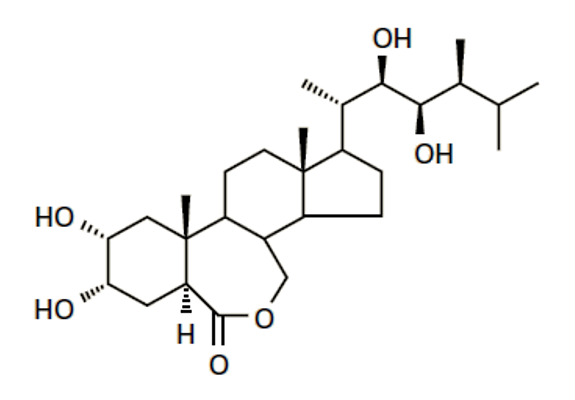
\includegraphics[width=.9\linewidth]{Imagenes/BL}
		\caption{}
		\label{BL}
	\end{subfigure}
	\begin{subfigure}{.4\textwidth}
		\centering
		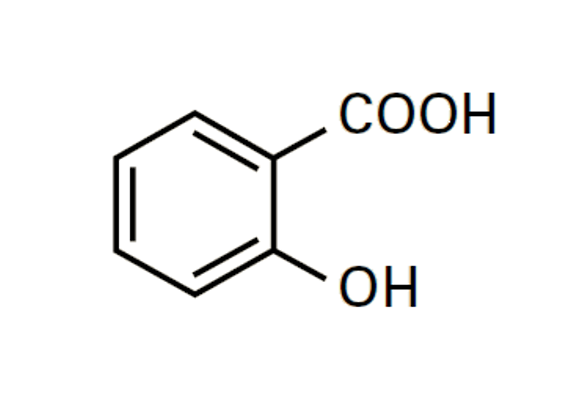
\includegraphics[width=.8\linewidth]{Imagenes/AS}
		\caption{}
		\label{AS}
	\end{subfigure}
	\caption{Estructura de hormonas vegetales, modificado de \cite{buchanan2015biochemistry} \\ a) Brasin\'olida (BL) y b) \'Acido salic\'ilico (AS).}
	\label{hormonas}
\end{figure}

La BL está considerada como el brasinoesteroide natural más activo descubierto hasta la fecha \citep{grove1979brassinolide}. Desafortunadamente, su concentración en fuentes naturales es baja, y tanto su purificación de fuentes vegetales como su síntesis orgánica constituye un proceso bastante costoso \citep{moreno2018silico}. Por tanto, se han buscado otras alternativas basadas en la síntesis de nuevas moléculas con alto grado de actividad biológica con bajos costos de producción \citep{lei2017structure}.\\

En este sentido, el laboratorio de Bioproductos del Centro de Investigación de Productos Naturales (CNPR) de la Facultad de Química de la Universidad de la Habana, ha desarrollado diversos productos a partir de saponinas y fitoesteroles de plantas, y mediante ensayos de actividad biológica se ha observado que algunos de estos tienen efectos naturales similares a BRs \citep{moreno2018silico}. Se analizaron, mediante métodos computacionales, la afinidad y las formas de unión de estos compuestos sintéticos análogos de BRs a su receptor BRI1 e indicaron que 17 de ellos pueden ser considerados buenos candidatos para la realización de pruebas biológicas. Entre estos análogos funcionales se destacan dos compuestos, DI-31 y MH-5 (Fig. \ref{br}), que han arrojado resultados prometedores en el efecto de estos compuestos en la defensa de las plantas frente al ataque por patógenos.\\

\begin{figure}[h!!!!]
	\begin{subfigure}{.5\textwidth}
		\centering
		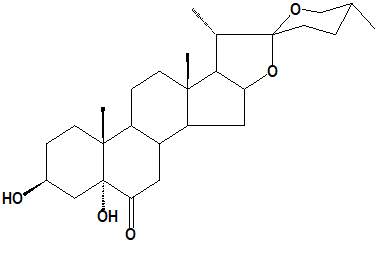
\includegraphics[width=.8\linewidth]{Imagenes/DI-31}
		\caption{}
		\label{di}
	\end{subfigure}
	\begin{subfigure}{.5\textwidth}
		\centering
		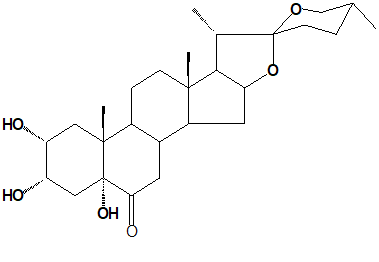
\includegraphics[width=.8\linewidth]{Imagenes/MH-5}
		\caption{}
		\label{mh}
	\end{subfigure}
	\caption{Estructura de an\'alogos sint\'eticos de BRs a) DI-31 y b) MH-5.}
	\label{br}
\end{figure}

\subsubsection{\'Acido salic\'ilico (AS).} 

El AS (Fig. \ref{AS}) es una hormona vegetal de naturaleza fen\'olica que participa en varias respuestas fisiol\'ogicas \citep{raskin1992salicylate} y se asocia con la activaci\'on de prote\'inas que participan en las respuestas de defensa \citep{glazebrook2005contrasting}.\\

En la literatura existen abundantes informes de la funci\'on del AS en la defensa contra distintos tipos de estr\'es abi\'otico, como los producidos por metales pesados \citep{alyemeni2014effect}, bajas temperaturas \citep{mutlu2013protective}, sequ\'ias \citep{alam2013exogenous} y salinidad \citep{fayez2014improving}, mediante el aumento de la actividad de las enzimas de defensa antioxidante. \\

\section{Especies reactivas del ox\'igeno (ROS).}

Las especies reactivas del ox\'igeno (ROS) son metabolitos del ox\'igeno molecular \citep{pandey2014oxidative}  que se generan en las plantas como consecuencia inevitable de las reacciones metab\'olicas aerobias \citep{buchanan2015biochemistry} o como respuesta de defensa. El ox\'igeno molecular es generalmente inactivo debido a la configuraci\'on de sus electrones \citep{elstner1987metabolism}, pero a diferencia de este, las ROS son mol\'eculas inestables y altamente reactivas. Entre las ROS se incluyen radicales del ox\'igeno: ani\'on super\'oxido $(O_{2}^{-} \bullet)$, radical hidroxilo $(OH\bullet)$ y radical perhidroxilo $(O_2H\bullet)$ y otras moléculas como el peróxido de hidrógeno $(H_2O_2)$ y el singlete de oxígeno $(^1O_2)$ \citep{buchanan2015biochemistry}.

\subsection{Producci\'on de ROS.}

En las plantas, la formaci\'on de ROS se lleva a cabo en diferentes compartimentos celulares \citep{apel2004reactive} e implica la fuga de electrones desde las cadenas transportadoras hacia el diox\'igeno \citep{corpas2015production}. Los cloroplastos y los peroxisomas son los principales productores en presencia de luz, mientras que la mitocondria es su principal fuente en condiciones de oscuridad \citep{choudhury2013reactive}. \\

El ani\'on super\'oxido se produce principalmente en  mitocondrias, apoplastos y en el fotosistema I (PSI) de los cloroplastos, mientras que el per\'oxido de hidr\'ogeno se genera en los peroxisomas \citep{gechev2006reactive, halliwell2006reactive}. \\

El singlete de ox\'igeno se produce principalmente en el fotosistema II de los cloroplastos. Su formación estimula la producción de  otras ROS \citep{buchanan2015biochemistry}, pero no se relaciona con la transferencia de electrones, ya que es el primer estado excitado del diox\'igeno, producido mediante fotoactivaci\'on \citep{triantaphylides2009singlet}. \\
 
%The chloroplast consists of a highly ordered system of thylakoids, which harbors the efficient light-capturing photosynthetic machinery. Photosystem (PS) I and PSII form the core of the light-harvesting systems in the thylakoids and are the primary sources of ROS generation [60, 61]. Near the reaction centers of PSII, O2 may produce 1O2 when there is overexcitation of chlorophyll under stress conditions. Besides, O2 •- may also be formed at PSI via Mehler reaction [62] or at PSII during electron transfer to O2 through QA and QB [55]. Additionally, due to the activities of flavin oxidases, peroxisomes are themain sites ofH2O2 generation [58, 63]. In mitochondria, O2 •- andH2O2 may be generated by univalent reduction of O2 near electron transport chain in plant cell [57]. 
%Apart from those organelles, there are cellular sites mediated in the generation of ROS. At plasmamembrane that plays a vital role in sensing environmental conditions, localized NADPH-dependent oxidase transfers electrons from NADPH on cytoplasmic side to O2 producing O2 •- [59]. ER also mediates the generation ofO2 •- by Cyt P450 [64].During harsh environmental conditions, the apoplast is rendered for H2O2 production by stress signals combined with ABA [65]. As cell wall localized peroxidase(s), diamine/polyamine oxidases and oxalate oxidase produceH2O2 that may, in turn, bemetabolized to OH• by the activity of class III peroxidases [66, 67]. 

Como se muestra en la figura \ref{ProdROS}, la reducción del $O_2$ ocurre a trav\'es de una secuencia de pasos. La primera reducción produce radicales superóxido o hidroperóxido. Posteriormente, el super\'oxido es dismutado a per\'oxido de hidr\'ogeno, lo cual puede ocurrir de forma espont\'anea (por p\'erdida de un electr\'on) o mediante la acci\'on de la enzima Super\'oxido Dismutasa (SOD) \citep{gechev2006reactive}. El per\'oxido de hidr\'ogeno producido puede ser transformado al radical hidroxilo en presencia de metales de transición como el hierro (Fe), mediante las reacciones de Haber-Weiss (o de Fenton) \citep{dat2000active}. Este tambi\'en puede ser eliminado por acción de la enzima catalasa (CAT) o del ciclo ascorbato-glutatión \citep{blokhina2003antioxidants, rinalducci2008redox}.\\

\begin{figure}[hbtp]
	\centering
	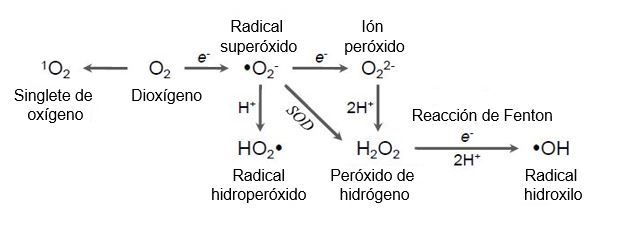
\includegraphics[scale=0.75]{Imagenes/ROSprod}
	\caption{Producci\'on de ROS durante la reducci\'on del ox\'igeno molecular. Modificado de \cite{imlay2008cellular, gill2010reactive}. }
	\label{ProdROS}
\end{figure}

\subsection{Efectos de ROS.}

Cuando los niveles de ROS son bajos o moderados funcionan como segundos mensajeros que median una serie de reacciones en las c\'elulas de las plantas, incluyendo el cierre de los estomas, la muerte celular programada (PCD, por sus siglas en ingl\'es) \citep{petrov2015ros}, gravitropismo \citep{wassim2013putative} y la adquisici\'on de tolerancia a estr\'es bi\'otico y abi\'otico \citep{nath2017reactive}. Pero el incremento de los niveles de ROS afecta una amplia variedad de funciones celulares, fisiol\'ogicas y bioqu\'imicas como la alteraci\'on de la membrana plasm\'atica, peroxidaci\'on lip\'idica, desnaturalizaci\'on de prote\'inas y destrucci\'on de ADN, ARN, enzimas y pigmentos \citep{xie2019roles}.\\
 
Aunque todas las ROS son muy reactivas, al poseer diferentes propiedades cada una puede reaccionar con diferentes biomol\'eculas \citep{peralta2012defensa}.\\

El ani\'on super\'oxido puede inactivar enzimas con centros hierro-azufre (Fe-S), mientras que el per\'oxido de hidr\'ogeno, aunque es relativamente estable, puede provocar la oxidación de grupos tiólicos e inactivar enzimas de esta manera. El radical perhidroxilo puede atravesar membranas y oxidar lípidos por la sustracción de protones de ácidos grasos poli-insaturados (PUFA). Por otra parte, el singlete de ox\'igeno es particularmente reactivo con dobles enlaces conjugados como los presentes en PUFA y aminoácidos aromáticos \citep{mittler2002oxidative, moller2007oxidative}.\\

Las propiedades tóxicas del super\'oxido y el per\'oxido de hidr\'ogeno aumentan en presencia de metales de transici\'on, ya que forman el radical hidroxilo que es la ROS más reactiva. Este radical tiene la capacidad de reaccionar rápidamente con todo tipo de macromoléculas y al no existir un mecanismo enzimático que la elimine, su sobreproducción finalmente conduce a la muerte de la c\'elula \citep{moller2007oxidative, sharma2009relationship, gill2010reactive}.\\

En cualquier caso, si la concentración intracelular de las ROS no es controlada, la consecuencia directa es el daño a estructuras celulares debido a la peroxidación de lípidos, oxidación de proteínas y componentes del ADN, así como la interrupción de rutas metabólicas \citep{moller2007oxidative, imlay2008cellular}.\\

\section{Estr\'es oxidativo.}

Existen v\'ias de eliminaci\'on que metabolizan las ROS y de esta forma controlan su concentraci\'on. Sin embargo, un desbalance en la generaci\'on y metabolismo de los niveles de ROS, interrumpe la homeostasis celular conduciendo a una variedad de retos fisiol\'ogicos que de forma general se conocen como \textquotedblleft estr\'es oxidativo\textquotedblright \citep{pandey2014oxidative}.\\

En las c\'elulas vegetales, el mayor da\~no oxidativo se produce en prote\'inas y l\'ipidos.  La actividad de las prote\'inas se altera mediante modificaciones en su estructura \citep{grimm2012oxidative}, mientras que los l\'ipidos, generalmente los poliinsaturados, pueden experimentar un proceso de descomposici\'on oxidativa en la membrana plasm\'atica, conocido como peroxidaci\'on lip\'idica \citep{catala2016impact, gaschler2017lipid}. Se ha demostrado que la peroxidaci\'on lip\'idica desencadena una serie de reacciones que producen otras mol\'eculas altamente reactivas, como cetonas, aldeh\'idos y mon\'oxido de hidr\'ogeno; adem\'as, puede modificar prote\'inas mediante la oxidaci\'on de algunos residuos aminoac\'idicos \citep{farmer2013ros, reginato2015role}.

\subsection{Mecanismos de resistencia}

Debido a los efectos da\~ninos que puede producir un desbalance de ROS, las plantas poseen un sistema de defensa antioxidante eficiente que evita el da\~no oxidativo y a la vez garantiza las funciones de se\~nalizaci\'on de las ROS \citep{liu2009oxidative, gill2010reactive}. Este sistema de defensa est\'a compuesto por mecanismos enzimáticos y no enzimáticos altamente regulados, que mantienen un balance entre la producción y eliminación de ROS, con el objetivo de mantener la homeostasis redox de la célula \citep{moller2001plant}.

\subsubsection{Mecanismos no enzim\'aticos}

Los antioxidantes no enzimáticos en plantas incluyen: ascorbato, glutati\'on reducido, taninos, flavonoides, $\alpha -$tocoferol, carotenoides y precursores de la lignina \citep{apel2004reactive}, que act\'uan a trav\'es de una serie de reacciones redox y evitan el da\~no oxidativo \citep{blokhina2003antioxidants}.\\

Los carotenoides y flavonoides neutralizan algunas ROS, entre las que se incluyen el per\'oxido de hidr\'ogeno y el singlete de ox\'igeno. El ascorbato es el antioxidante hidrosoluble m\'as abundante y poderoso que protege las membranas. El glutatión reducido constituye un importante mecanismo antioxidante y est\'a involucrado en algunas funciones vitales dentro de la c\'elula \citep{mittler2002oxidative}. El $\alpha-$tocoferol es el principal antioxidante liposoluble en las membranas fotosint\'eticas donde protege contra la peroxidaci\'on lip\'idica \citep{gechev2006reactive}. 

\subsubsection{Mecanismos enzim\'aticos}

Los mecanismos enzimáticos incluyen a las enzimas superóxido dismutasa (SOD), catalasa (CAT), ascorbato peroxidasa (APX), monodihidroascorbato reductasa (MDHAR), guaiacol peroxidasa (POX), glutatión reductasa (GR) y glutati\'on peroxidasa (GPX) \citep{ruley2004antioxidant}. \\

La SOD constituye la primera línea de defensa contra las ROS y es la \'unica enzima en plantas que dismuta el ani\'on super\'oxido en per\'oxido de hidr\'ogeno. El per\'oxido de hidr\'ogeno puede ser directamente catabolizado por CAT, o en presencia de sustratos reductores por varios tipos de peroxidasas, en el ciclo ascorbato$-$glutati\'on \citep{halliwell2006reactive}.\\

La extensión del estrés oxidativo en una célula está determinada por la cantidad de superóxido, per\'oxido de hidr\'ogeno y radicales hidroxilo. Por lo tanto, el balance de las actividades de SOD y CAT es crucial para suprimir los niveles tóxicos de ROS en la célula \citep{benezer2008produccion}. \\

\section{Enzimas de defensa en plantas.}

\subsection{Super\'oxido Dismutasa (SOD) (EC 1.15.1.1).}

Las Superóxido Dismutasas son una familia de metaloenzimas, descritas por primera vez por \cite{mccord1969superoxide}, que constituyen la primera línea de defensa antioxidante contra las ROS, catalizando la reacci\'on:
$$2O_2^- \; + \; 2H^+ \; \longrightarrow \; H_2O_2 \; + \; O_2$$

Existen tres isoformas de la enzima que son clasificadas de acuerdo al i\'on met\'alico presente en el centro activo: cobre/zinc (SOD Cu/Zn), hierro (SOD Fe) y manganeso (SOD Mn). Estas isoenzimas est\'an distribuidas en diferentes compartimentos celulares, probablemente porque el ani\'on super\'oxido no puede difundir a trav\'es de las membranas \citep{takahashi1983superoxide}, por lo que debe ser eliminado en su sitio de producci\'on. La comparaci\'on de las secuencias y estructuras de estas isoformas indican que SOD Mn y SOD Fe están estrechamente relacionadas, mientras SOD Cu/Zn parecen haber evolucionado independientemente \citep{bowler1994superoxide}.\\

La isoforma SOD Cu/Zn es la más abundante en organismos eucariotas y está localizada principalmente en el citoplasma, en los cloroplastos y en diferentes tipos de peroxisomas. También se encuentran en el núcleo y en el apoplasto. La isoforma SOD Mn se ha encontrado en mitocondrias y peroxisomas, mientras que la isoforma SOD Fe está presente en los cloroplastos \citep{munoz2005crystal}.\\

Para cada isoforma el mecanismo de cat\'alisis es similar e involucra un bolsillo o pliegue rodeado de residuos aminoac\'idicos cargados positivamente que atraen al ani\'on super\'oxido hacia el centro activo de la enzima. El metal de transici\'on presente en el centro activo lleva a cabo una transferencia de electrones entre dos aniones super\'oxido \citep{bowler1994superoxide}. \\

\subsection{Catalasa (CAT) (EC 1.11.1.6).}

La catalasa ($H_2O_2$:$H_2O_2$ oxidorreductasa) es una hemoprote\'ina tetram\'erica que est\'a presente en la mayor\'ia de los organismos aerobios. Adem\'as, es una de las enzimas principales en el catabolismo del per\'oxido de hidr\'ogeno \citep{luhova2003activities}. \\

Las CAT de plantas se encuentran mayormente en los peroxisomas \citep{luhova2003activities} y existen varias isoformas de la enzima, lo que sugiere que posee m\'ultiples funciones \citep{scandalios1997catalases}.\\

En dependencia de la concentraci\'on de per\'oxido de hidr\'ogeno, la CAT puede ejercer una funci\'on dual \citep{deisseroth1970catalase}. A bajas concentraciones puede actuar peroxidativamente, donde varias sustancias como el etanol y el \'acido asc\'orbico pueden ser oxidadas siguiendo la reacci\'on:

$$RH_2 \; +\; H_2O_2 \; \rightarrow \; R \; + \; 2H_2O $$

Mientras que a altas concentraciones de sustrato la CAT descompone r\'apidamente el per\'oxido de hidr\'ogeno mediante la reacci\'on catal\'itica:

$$2H_2O_2 \; \rightarrow \; 2H_2O \; + \; O_2$$

Evidencias cin\'eticas y espectrofotom\'etricas sugieren que la CAT utiliza un mecanismo de dos pasos en estas reacciones \citep{deisseroth1970catalase, dounce1983proposed}. \\

En la reacci\'on catal\'itica, la CAT presenta una constante de Michaelis-Menten muy elevada, en consecuencia, la enzima no se satura f\'acilmente con sustrato. De esta manera, la actividad enzim\'atica aumenta linealmente frente a una amplia gama de concentraciones de per\'oxido de hidr\'ogeno, lo que le permite controlar la concentraci\'on intracelular de esta ROS \citep{scandalios1997catalases}.\\




\subsection{Polifenol oxidasa (PPO) (EC 1.10.3.1).}

Las PPO son una familia de metaloenzimas monom\'ericas que reaccionan con una amplia gama de sustratos fen\'olicos. El centro activo de la enzima consiste en dos \'atomos de cobre, cada uno acoplado con tres residuos de histidina conservados \citep{lerch1983neurospora, huber1985primary}.\\

Las PPO se encuentran en la membrana de los tilacoides de los cloroplastos  y son liberadas al citoplasma ante daños mecánicos en la estructura tisular y celular que pueden ocurrir durante la senescencia, lesiones o estr\'es \citep{marshall2000enzymatic, mayer2006polyphenol}. Esto conduce al contacto de la enzima con compuestos fen\'olicos que son liberados desde la vacuola, donde se encuentran almacenados \citep{queiroz2008polyphenol}. La actividad catal\'itica de la enzima est\'a influenciada por caracter\'isticas estructurales de los sustratos, como la naturaleza de la cadena lateral y el n\'umero de grupos hidroxilo y la posici\'on que ocupan en el anillo de benzeno \citep{macheix1990phenolic}.\\

La PPO cataliza dos reacciones (Fig. \ref{PO}): la o-hidroxilaci\'on de monofenoles a o-difenoles (actividad creolasa) y la oxidaci\'on de estos a o-quinonas (actividad catecolasa), utilizando el oxígeno molecular como agente oxidante \citep{jukanti2017distribution}.\\

\begin{figure}[hbtp]
	\centering
	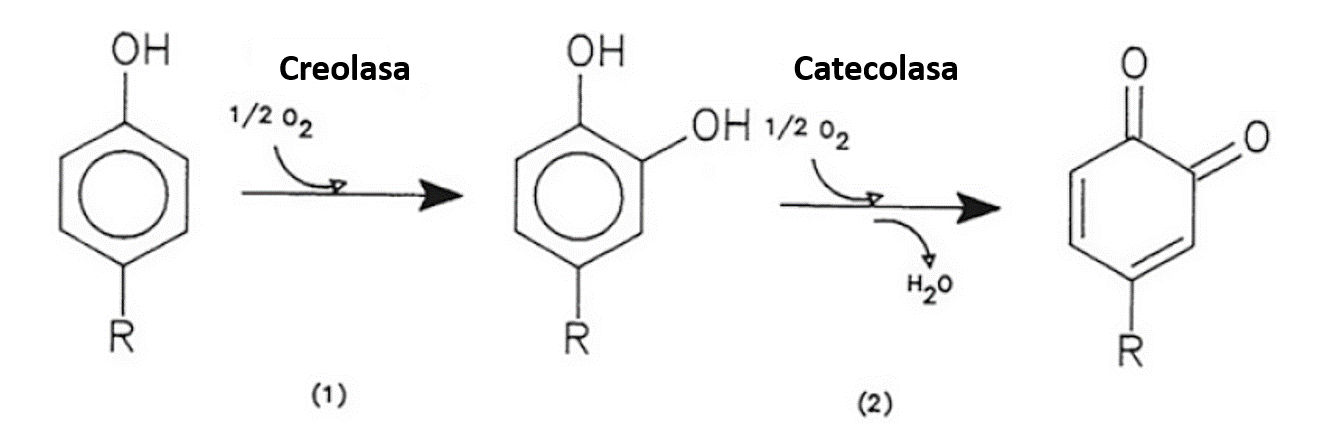
\includegraphics[scale=0.65]{Imagenes/PO}
	\caption{Actividad creolasa (1) y catecolasa (2) de PPO. Modificado de \cite{nicolas1994enzymatic}. }
	\label{PO}
\end{figure}

Las o-quinonas generadas son altamente reactivas e inestables \citep{mayer2006polyphenol} y pueden reaccionar con grupos amino y tiol de aminoácidos libres y proteínas mediante mecanismos no enzimáticos, o reaccionar covalentemente con otros compuestos fenólicos para formar diferentes pigmentos, ocasionando así el efecto conocido como pardeamiento enzimático \citep{kumar2008purification}. Este efecto es muy com\'un en frutas y verduras y ha sido propuesto como mecanismo de defensa contra pat\'ogenos e insectos \citep{mayer1979polyphenol, vaughn1988polyphenol}.\\

Las PPO han sido implicadas en las respuestas de defensa de las plantas debido a la aparici\'on de sus productos de reacci\'on en el momento de ataques de pat\'ogenos e insectos, lesiones y diferentes tipos de estr\'es \citep{mayer1979polyphenol, constabel1995systemin, maki2006development}. Adem\'as, se ha identificado que aplicaciones ex\'ogenas de BRs aumentan la tolerancia de plantas a diferentes tipos de estr\'es, mediante el incremento de la actividad de PPO \citep{sharma2010regulation, sharma2012effect, el2012brassinolide}.\\

\section{Par\'ametros experimentales.}

En la figura \ref{curva} se muestra la velocidad máxima inicial ($V_{max}$) a una concentración determinada de enzima $[E_o]$. Este par\'ametro cin\'etico posee las mismas unidades de v$_o$ y representa la máxima eficiencia catalítica de una enzima frente a un sustrato específico, a la concentración de enzima y valores de pH, fuerza iónica y temperatura utilizados experimentalmente \citep{chavez1990temas}.\\

\begin{figure}[hbtp]
	\centering
	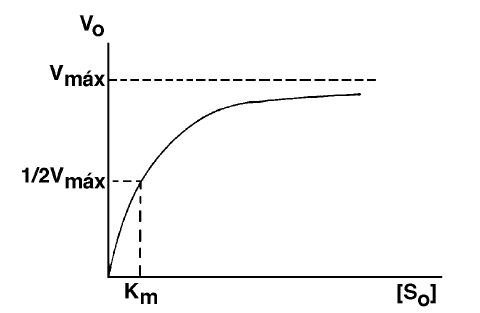
\includegraphics[scale=0.8]{Imagenes/curva}
	\caption{Representación gráfica de v$_o$ en función de $[S_o]$, a $[E_o]$ constante, para una reacción enzimática monosustrato, a partir de la ecuación de Michaelis-Menten. $V_{max}$: velocidad máxima; $K_m$: constante de Michaelis \citep{chavez1990temas}.}
	\label{curva}
\end{figure}

En la figura \ref{curva} también se muestra el valor de $K_m$. Este par\'ametro cin\'etico representa la concentración inicial de sustrato $[S_o]$, que da lugar a una velocidad inicial igual a la mitad de la velocidad máxima y tiene las mismas unidades de $[S_o]$. El valor de $K_m$ es característico de una enzima frente a un sustrato particular y en las condiciones de pH, fuerza iónica y temperatura del experimento, pero no depende de la concentración de enzima \citep{chavez1990temas}.\\

El valor de $K_m$ medido de esta forma puede diferir de su valor verdadero, el cual es definido en términos de constantes de velocidad. Si hay presente inhibidores u otros factores, el valor medido debe ser denominado $K_m \; aparente$ \citep{chavez1990temas}. \\

En las condiciones de cumplimiento del equilibrio de Michaelis-Menten, cuando $K_m$ = $K_s$ el valor de $K_m$ puede reflejar la mayor o menor afinidad de una enzima por un sustrato. Esta relación es inversa, por tanto, a mayor valor de $K_m$ más concentración de sustrato se requiere para alcanzar la mitad de $V_{max}$ y viceversa \citep{chavez1990temas}.\\

%%KM es una constante de disociación aparente que puede ser tratada como una constante global de disociación de todos los complejos enzimáticos intermediarios\citep{chavez1990temas}.

%ks constante de saturaci\'on

En este trabajo, no es posible determinar la $K_{cat}$ debido a que la enzima no est\'a purificada, por lo que se trabajar\'a con $V_{max}$ . Por este motivo, tampoco se puede determinar el valor real de $K_m$, por lo que el valor obtenido para este par\'ametro ser\'a referido como $K_ma$ y ser\'a utilizado para caracterizar las enzimas. \\

%Evaluaremos la afinidad de las enzimas por el sustrato
%
%1- La constante de Michaelis-Menten es un elemento de juicio importante para caracterizar una enzima.
%2- El Km indica la afinidad de la enzima por el sustrato. 


\section{\textit{Raphanus sativus} como modelo experimental.}

La selecci\'on de este modelo experimental se basa en el gran n\'umero de fuentes existentes en la literatura, donde son utilizadas plantas de r\'abano para estudiar el efecto de BRs en las enzimas de defensa vegetal. El r\'abano es considerado un cultivo modelo para el estudio de los efectos de distintos tipos de estr\'es, entre ellos h\'idrico  \citep{mahesh2013effect}, oxidativo \citep{sharma2012effect} y por metales pesados \citep{dhriti201424}. \\

Las plantas de r\'abano poseen un tiempo relativamente corto de germinaci\'on, as\'i como un bajo costo, lo que constituyen ventajas en su utilizaci\'on como modelo experimental. Adem\'as, numerosos estudios han corroborado el aumento de las enzimas de defensa de \textit{Raphanus sativus} al aplicar an\'alogos sint\'eticos de BRs. 

